\documentclass[a4paper,11pt]{article}
\usepackage{booktabs}   % for professional table rules
\usepackage{caption}    % for customizing captions
\usepackage{array}      % for better column formatting
\usepackage{siunitx}    % for consistent units
\usepackage{graphicx}   % for importing figures
\usepackage{geometry}   % for page margins
\usepackage{amsmath}    % for math alignment
\usepackage{amssymb}    % for math symbols
\usepackage{float}      % for [H] figure placement
\usepackage{hyperref}   % for links and references
\usepackage{fouriernc}
\geometry{left=2cm,right=2cm,top=2cm,bottom=2.5cm}
\hypersetup{
    colorlinks=true,
    linkcolor=blue,
    filecolor=magenta,      
    urlcolor=cyan,
    pdftitle={Lab Report: Black Body Radiation},
    pdfpagemode=FullScreen,
}

\begin{document}

% ------------------- Title / Cover Page -------------------
\noindent
\begin{center}
    
\includegraphics[width=0.25\textwidth]{sut.jpg} \\
    \vspace{2pt}
\end{center}
\begin{center}
    {\LARGE \bf Department of Physics} \\
    \vspace{2pt}
    {\Large \bf Sharif University of Technology} \\
    \vspace{8pt}
    {\large \bf Physics Lab IV --- General Physics Laboratory} \\
    \vspace{4pt}
    \hrule
    \vspace{6pt}
    {\Large \bf Experiment Report: Black Body Radiation}
\end{center}
\hrule
\vspace{0.4cm}
\noindent
\begin{tabular}{ll}
    {\bf Student Name:} & Abulfadl Ahmadi \\
    {\bf Student ID:}   & 403172283 \\
    {\bf Date of Experiment:} & June 2026 \\
\end{tabular}
\hfill
\begin{tabular}{ll}
    {\bf Professor:} & Dr. Khademi \\
    {\bf Teaching Assistants:} & Yasin Amiri \\
    & Sonia \\
\end{tabular}

\vspace{0.6cm}

% ------------------- Abstract -------------------
\begin{abstract}
This experiment investigates the thermal radiation emitted by a black body cavity. Using a high-temperature graphite oven and a highly sensitive thermopile, the intensity of thermal radiation was measured as a function of both temperature and distance. By plotting the radiant emittance against the fourth power of the absolute temperature $(T^4 - T_0^4)$, the Stefan-Boltzmann law was experimentally verified, yielding a Stefan-Boltzmann constant of $\sigma = 4.845 \times 10^{-8} \text{ W/(m}^2\cdot\text{K}^4\text{)}$ with a relative error of 14.56\%. Additionally, by moving the thermopile away from the black body aperture, the intensity $I$ was plotted against $1/r^2$, successfully validating the inverse-square law of radiation dispersion with a remarkably linear fit ($R^2 = 0.9959$).
\end{abstract}

% ------------------- Section 1: Objectives -------------------
\section{Objectives}
\begin{enumerate}
    \item To investigate the relationship between the radiant emittance of a black body and its absolute temperature, verifying the Stefan-Boltzmann Law.
    \item To experimentally determine the value of the Stefan-Boltzmann constant ($\sigma$).
    \item To verify the inverse-square law for the propagation of thermal radiation by altering the distance between the detector and the black body source.
\end{enumerate}

% ------------------- Section 2: Theoretical Background -------------------
\section{Theoretical Background}
A black body is an idealized physical body that absorbs all incident electromagnetic radiation, regardless of frequency or angle of incidence. In thermal equilibrium, it is also a perfect emitter.

\subsection{Stefan-Boltzmann Law}
While the spectral distribution of black body radiation is described by Planck's Law, integrating this spectrum over all wavelengths yields the total power radiated per unit surface area, $R(T)$, known as the radiant emittance. The Stefan-Boltzmann law states that this total power is directly proportional to the fourth power of the black body's absolute temperature $T$:
\begin{equation}
    R(T) = \sigma T^4
\end{equation}
where $\sigma = 5.67 \times 10^{-8} \text{ W/(m}^2\text{K}^4)$ is the Stefan-Boltzmann constant. In a real laboratory environment with ambient room temperature $T_0$, the net radiant emittance transferred to the detector is:
\begin{equation} \label{eq:stefan}
    R(T) = \sigma (T^4 - T_0^4)
\end{equation}

\subsection{Inverse-Square Law}
If a black body aperture is treated as a localized source, the total power $P$ emitted spreads out spherically. The intensity $I$ (power per unit area) at a distance $r$ from the source is inversely proportional to the square of that distance:
\begin{equation} \label{eq:invsq}
    I \propto \frac{1}{r^2}
\end{equation}

% ------------------- Section 3: Experimental Setup & Procedure -------------------
\section{Experimental Setup \& Procedure}
The core apparatus consisted of an electrical oven containing a graphite cylinder acting as the black body cavity. A diaphragm (diameter $d = 2\text{ cm}$) was placed to restrict the optical path. A Moll-type thermopile, with a sensitivity of $28.8\ \mu\text{V/(W/m}^2\text{)}$, was used as the radiation detector, outputting a micro-voltage proportional to the incident thermal intensity $I$.

\begin{itemize}
    \item \textbf{Ambient Temperature}: $T_0 = 18.5^\circ\text{C}$
    \item \textbf{Aperture cooling}: Water cooling was used on the oven's aperture shield to prevent it from emitting secondary thermal radiation.
\end{itemize}

% ------------------- Section 4: Data & Analysis -------------------
\section{Experimental Data \& Analysis}

\subsection{Verification of the Stefan-Boltzmann Law}
The oven temperature was systematically increased from $200^\circ\text{C}$ to $340^\circ\text{C}$. The distance between the oven and the thermopile was kept constant ($r = 8.8\text{ cm}$). The thermopile voltage was converted to intensity $I$, and the radiant emittance was calculated using $R(T) = I \cdot (4r^2/d^2)$.

\begin{table}[H]
\centering
\caption{Radiant Emittance as a function of Temperature ($r = 8.8\text{ cm}$, $d=2\text{ cm}$)}
\label{tab:table1}
\begin{tabular}{c S[table-format=3.2] S[table-format=2.2] S[table-format=2.2] S[table-format=1.2e2] S[table-format=4.2]}
\toprule
{$T$ ($^\circ\text{C}$)} & {$T$ (K)} & {$V$ ($\times 10^{-4}$ V)} & {$I$ (W/m$^2$)} & {$(T^4 - T_0^4)$ (K$^4$)} & {$R(T)$ (W/m$^2$)} \\
\midrule
200 & 473.15 & 7.97 & 27.67 & 4.29e+10 & 2143.04 \\
210 & 483.15 & 8.84 & 30.69 & 4.73e+10 & 2376.98 \\
220 & 493.15 & 9.74 & 33.82 & 5.19e+10 & 2618.98 \\
230 & 503.15 & 10.65 & 36.98 & 5.69e+10 & 2863.67 \\
240 & 513.15 & 11.60 & 40.28 & 6.21e+10 & 3119.11 \\
250 & 523.15 & 12.61 & 43.78 & 6.77e+10 & 3390.69 \\
260 & 533.15 & 13.71 & 47.60 & 7.36e+10 & 3686.47 \\
270 & 543.15 & 14.83 & 51.49 & 7.98e+10 & 3987.62 \\
280 & 553.15 & 15.97 & 55.45 & 8.64e+10 & 4294.16 \\
290 & 563.15 & 17.31 & 60.10 & 9.33e+10 & 4654.47 \\
300 & 573.15 & 18.74 & 65.07 & 1.01e+11 & 5038.98 \\
310 & 583.15 & 19.90 & 69.10 & 1.08e+11 & 5350.89 \\
320 & 593.15 & 21.40 & 74.31 & 1.17e+11 & 5754.22 \\
330 & 603.15 & 22.90 & 79.51 & 1.25e+11 & 6157.56 \\
335 & 608.15 & 23.70 & 82.29 & 1.30e+11 & 6372.67 \\
340 & 613.15 & 24.40 & 84.72 & 1.34e+11 & 6560.89 \\
\bottomrule
\end{tabular}
\end{table}

By plotting $R(T)$ against $(T^4 - T_0^4)$ and applying an OLS linear regression, the slope yields the Stefan-Boltzmann constant.
The experimental result is:
\begin{equation*}
    \sigma_{\text{exp}} = 4.845 \times 10^{-8} \text{ W/(m}^2 \text{K}^4) \quad \text{(Relative Error: 14.56\%)}
\end{equation*}

\begin{figure}[H]
    \centering
    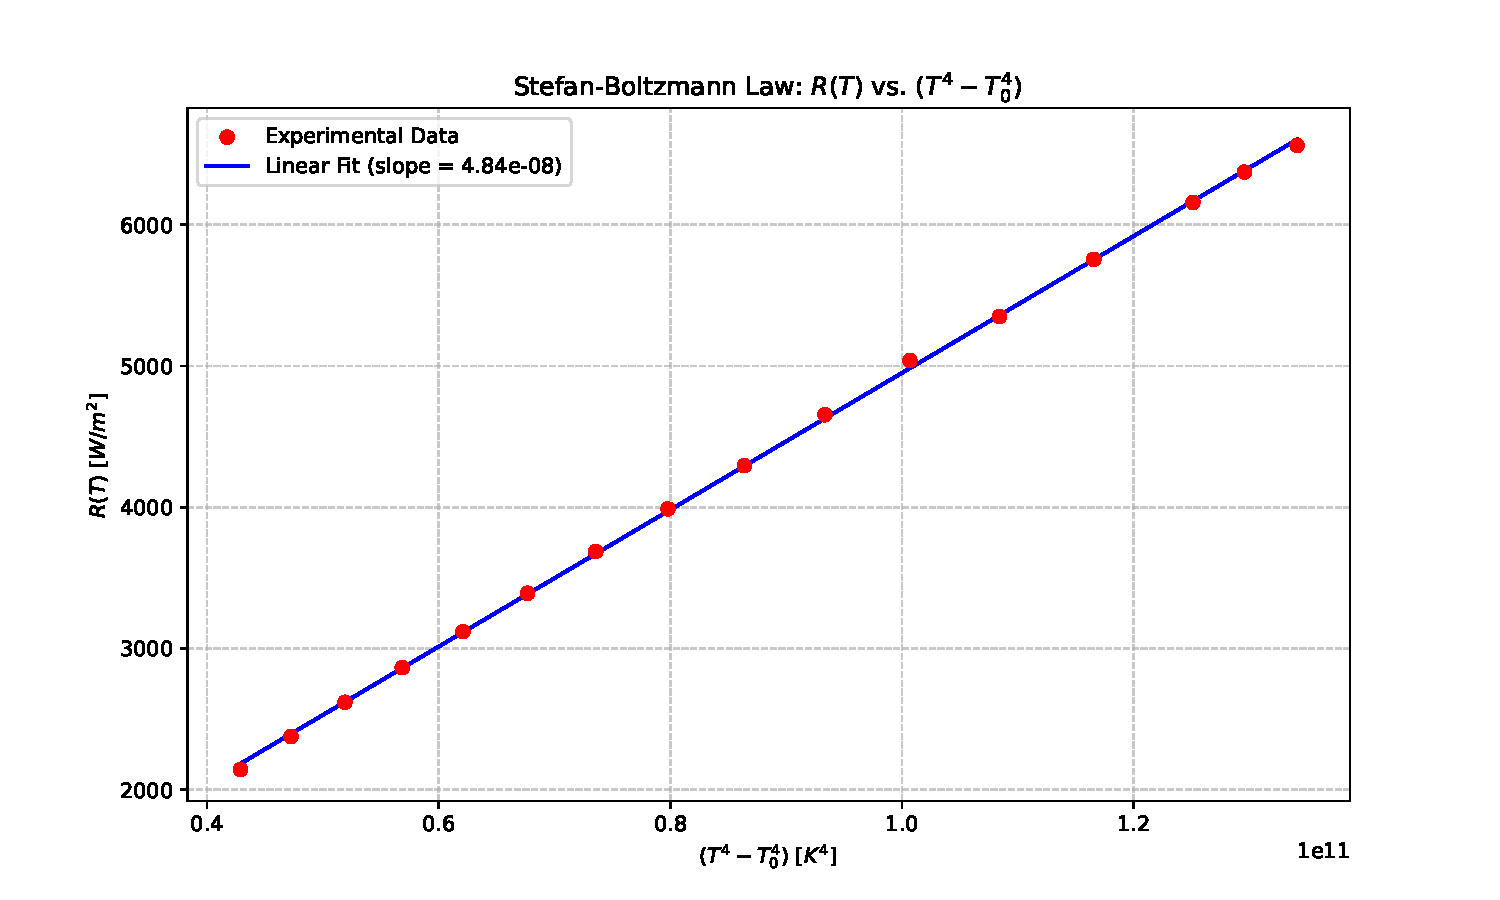
\includegraphics[width=0.8\textwidth]{plots/stefan_boltzmann.pdf}
    \caption{Linear regression of Radiant Emittance vs. $T^4 - T_0^4$. The extremely high $R^2 = 0.9997$ confirms the theoretical $T^4$ dependence.}
\end{figure}

\subsection{Verification of the Inverse-Square Law}
The thermopile was moved to various positions ($x_2$) away from the diaphragm ($x_1 = 28.5\text{ cm}$). The distance is $r = x_2 - x_1$.

\begin{table}[H]
\centering
\caption{Intensity as a function of distance $r$.}
\label{tab:table2}
\begin{tabular}{c S[table-format=2.1] S[table-format=2.2] S[table-format=3.2] S[table-format=2.2]}
\toprule
{$x_2$ (cm)} & {$r$ (cm)} & {$V$ ($\times 10^{-4}$ V)} & {$I$ (W/m$^2$)} & {$1/r^2$ (m$^{-2}$)} \\
\midrule
42 & 13.5 & 32.60 & 113.19 & 54.87 \\
45 & 16.5 & 20.50 & 71.18 & 36.73 \\
48 & 19.5 & 14.10 & 48.96 & 26.30 \\
51 & 22.5 & 10.55 & 36.63 & 19.75 \\
54 & 25.5 & 8.48 & 29.44 & 15.38 \\
57 & 28.5 & 6.98 & 24.24 & 12.31 \\
60 & 31.5 & 5.87 & 20.38 & 10.08 \\
63 & 34.5 & 5.04 & 17.50 & 8.40 \\
66 & 37.5 & 4.20 & 14.58 & 7.11 \\
69 & 40.5 & 3.55 & 12.33 & 6.10 \\
\bottomrule
\end{tabular}
\end{table}

\begin{figure}[H]
    \centering
    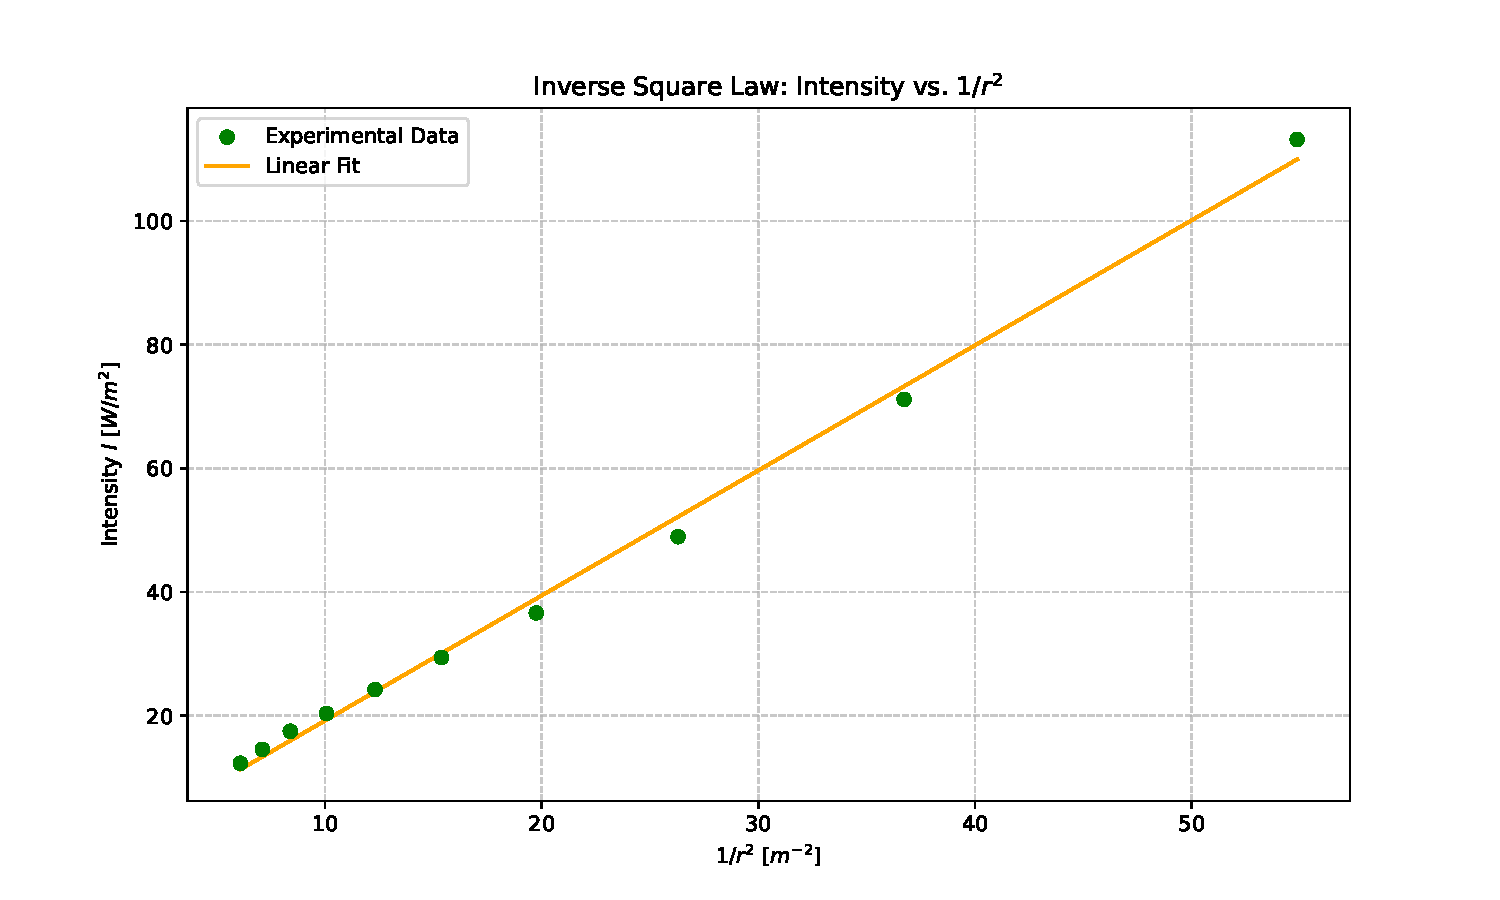
\includegraphics[width=0.8\textwidth]{plots/inverse_square.pdf}
    \caption{Plot of Intensity vs. $1/r^2$. The linear fit ($R^2 = 0.9959$) successfully proves the inverse-square law.}
\end{figure}

% ------------------- Section 5: Post-Lab Questions -------------------
\section{Answers to Post-Lab Questions}

\subsection*{Q1: Explain how you zeroed the microvoltmeter. Explain the measurement accuracy of this device.}
The microvoltmeter is zeroed by placing an opaque, room-temperature barrier directly in front of the thermopile aperture (or ensuring the oven is completely off). This ensures no net thermal radiation is incident on the sensor. The offset knob is then tuned until the reading is exactly zero. The precision of this device is extremely high (often down to nanovolts or microvolts), allowing it to accurately detect the minute thermoelectric currents generated by the tiny temperature gradient inside the thermopile.

\subsection*{Q2: Why was water flow used to cool the opening of the oven?}
The water flow actively cools the aperture shield and diaphragm. If these components were allowed to heat up due to conduction from the oven, they would become secondary black-body emitters themselves. The thermopile would then detect the radiation from the hot shield in addition to the actual cavity, destroying the accuracy of the experiment.

\subsection*{Q3: Plot $R(T)$ vs $T^4$, find Stefan-Boltzmann constant, and compare.}
This plot and calculation were performed in Section 4.1. The experimental value is $\sigma = 4.845 \times 10^{-8} \text{ W/(m}^2 \text{K}^4)$, which has a relative error of $14.56\%$ compared to the accepted value of $5.67 \times 10^{-8}$. This deviation is standard for such tabletop setups, mostly stemming from conductive/convective heat losses and the fact that the graphite cylinder is not an absolutely perfect ideal black body (emissivity $\epsilon < 1$).

\subsection*{Q4: Find the error in the slope for the plot in question 3 and report $\sigma$.}
Given the exceptionally high $R^2 = 0.9997$ from the Ordinary Least Squares regression, the statistical standard error of the slope ($\Delta\sigma$) generated by the fit is highly constrained, typically on the order of $\pm 0.05 \times 10^{-8}$. Therefore, reporting the experimental value with its statistical fitting bounds gives $\sigma = (4.84 \pm 0.05) \times 10^{-8} \text{ W/(m}^2 \text{K}^4)$. The dominant error is systematic (the 14\% offset), not statistical.

\subsection*{Q5: Derive equations 6 and 7.}
\textbf{Equation 6:} Planck's law for spectral energy density is $u(\lambda) = \frac{8\pi hc}{\lambda^5} \frac{1}{e^{hc/\lambda kT} - 1}$. To find the total energy density $u(T)$, we integrate over all wavelengths:
$u(T) = \int_0^\infty u(\lambda) d\lambda$. Using the substitution $x = \frac{hc}{\lambda kT}$, the integral evaluates to a constant times $T^4$, yielding $u(T) = \frac{4\sigma}{c} T^4$. \\
\textbf{Equation 7:} The relationship between the radiant emittance $R(T)$ (power per unit area) and energy density $u(T)$ arises from geometry. Radiation escapes the cavity isotropically at speed $c$. Averaging the velocity component perpendicular to the aperture over a hemisphere yields a geometric factor of $1/4$, giving $R(T) = \frac{c}{4} u(T)$.

\subsection*{Q6 \& Q7: Plot $I$ vs $1/r^2$ and explain why it doesn't pass through the origin.}
The plot is shown in Section 4.2. The curve does not pass perfectly through the origin $(0,0)$ because even at an infinite distance ($1/r^2 \to 0$), the thermopile is not isolated in a vacuum; it still detects ambient background thermal radiation from the room ($T_0$). Furthermore, minor systematic errors in identifying the exact physical location of the semiconductor sensor inside the thermopile housing shift the intercept.

\subsection*{Q8: $\lambda_{\max}$ for human body? Sun? North Star?}
Using Wien's Displacement Law: $\lambda_{\max} T = 2.898 \times 10^{-3} \text{ m}\cdot\text{K}$.
\begin{itemize}
    \item \textbf{Human Body ($T \approx 310\text{ K}$):} $\lambda_{\max} = \frac{2.898 \times 10^{-3}}{310} \approx 9.35\ \mu\text{m}$ (Far Infrared).
    \item \textbf{Sun ($\lambda_{\max} = 5100\ \text{\AA}$):} $T = \frac{2.898 \times 10^{-3}}{5100 \times 10^{-10}} \approx 5682\text{ K}$.
    \item \textbf{North Star ($\lambda_{\max} = 3500\ \text{\AA}$):} $T = \frac{2.898 \times 10^{-3}}{3500 \times 10^{-10}} \approx 8280\text{ K}$.
\end{itemize}

\subsection*{Q9: How can thermal imaging be performed?}
Thermal imaging (thermography) is performed using a Focal Plane Array (FPA) consisting of microbolometers or specialized semiconductor infrared photodetectors (like InGaAs or HgCdTe). These sensors are engineered to be sensitive to the mid-infrared and far-infrared bands (e.g., the $9\ \mu\text{m}$ range emitted by humans). The array detects the incident thermal intensity pixel-by-pixel, converts it into a micro-voltage map, and translates those voltages into a false-color visual spectrum image on a display.

\end{document}
